% ============================================================================
%  Naive baseline space-time diagram (companion "before" figure)
%  paired with pipeline_spacetime.tex (the optimised "after" figure)
%
%  Build:      pdflatex naive_pipeline.tex
%  Output:     naive_pipeline.pdf   (standalone, crop-fit)
% ============================================================================
\documentclass[tikz,border=4pt]{standalone}

\usepackage{mathpazo}      % paper-style Palatino text + math
\usepackage{inconsolata}   % matching monospaced font
\usepackage{amsmath,amssymb}
\usepackage{xcolor}
\usepackage{tikz}
\usetikzlibrary{positioning,arrows.meta,calc,fit,backgrounds,decorations.pathreplacing,patterns,shadows.blur}

% --------------------- paper-grade palette (muted, colour-blind safe) -------
\definecolor{hbmC}  {HTML}{4C78A8}   % HBM load         (steel blue)
\definecolor{smC}   {HTML}{F58518}   % SMEM prefetch    (amber)
\definecolor{tcC}   {HTML}{D62728}   % INT4 Tensor Core (crimson)
\definecolor{fpC}   {HTML}{2CA02C}   % FP32 epilogue    (green)
\definecolor{spC}   {HTML}{9467BD}   % sparse branch    (purple)
\definecolor{qC}    {HTML}{7F7F7F}   % activation quant (neutral grey)
\definecolor{redC}  {HTML}{17A2B8}   % reduce_sum       (teal, distinct from fp green)
\definecolor{stallC}{HTML}{BAB0AC}   % idle / sync stall (warm grey)
\definecolor{axisC} {HTML}{1F2933}   % axes + text
\definecolor{ghostC}{HTML}{D3D3D3}
\definecolor{hlC}   {HTML}{FFF1C1}   % yellow highlight band
\definecolor{rtC}   {HTML}{C44E52}   % HBM round-trip arrow

% --------------------- TikZ styles ------------------------------------------
\tikzset{
  >=Latex,
  font=\small,
  every node/.style={font=\small},
  lane/.style={draw=axisC!30, thin},
  lanelab/.style={font=\footnotesize, align=right, anchor=east, text=axisC},
  % four phase-block palettes
  blkQ/.style   ={draw=qC!70!black,   fill=qC!22,    rounded corners=1.4pt,
                  minimum height=7.5mm, inner sep=2pt, font=\scriptsize,
                  blur shadow={shadow blur steps=4, shadow blur extra rounding=.4pt,
                               shadow xshift=.3pt, shadow yshift=-.3pt, shadow opacity=22}},
  blkHBM/.style ={draw=hbmC!70!black, fill=hbmC!25,  rounded corners=1.4pt,
                  minimum height=7.5mm, inner sep=2pt, font=\scriptsize,
                  blur shadow={shadow blur steps=4, shadow blur extra rounding=.4pt,
                               shadow xshift=.3pt, shadow yshift=-.3pt, shadow opacity=22}},
  blkTC/.style  ={draw=tcC!70!black,  fill=tcC!22,   rounded corners=1.4pt,
                  minimum height=7.5mm, inner sep=2pt, font=\scriptsize,
                  blur shadow={shadow blur steps=4, shadow blur extra rounding=.4pt,
                               shadow xshift=.3pt, shadow yshift=-.3pt, shadow opacity=22}},
  blkFP/.style  ={draw=fpC!70!black,  fill=fpC!22,   rounded corners=1.4pt,
                  minimum height=7.5mm, inner sep=2pt, font=\scriptsize,
                  blur shadow={shadow blur steps=4, shadow blur extra rounding=.4pt,
                               shadow xshift=.3pt, shadow yshift=-.3pt, shadow opacity=22}},
  blkSP/.style  ={draw=spC!70!black,  fill=spC!22,   rounded corners=1.4pt,
                  minimum height=7.5mm, inner sep=2pt, font=\scriptsize,
                  blur shadow={shadow blur steps=4, shadow blur extra rounding=.4pt,
                               shadow xshift=.3pt, shadow yshift=-.3pt, shadow opacity=22}},
  blkRED/.style ={draw=redC!70!black, fill=redC!22,  rounded corners=1.4pt,
                  minimum height=7.5mm, inner sep=2pt, font=\scriptsize,
                  blur shadow={shadow blur steps=4, shadow blur extra rounding=.4pt,
                               shadow xshift=.3pt, shadow yshift=-.3pt, shadow opacity=22}},
  blkStall/.style={draw=stallC!60!black, fill=stallC!30, rounded corners=1pt,
                   minimum height=7.5mm, inner sep=1pt, font=\scriptsize\itshape,
                   pattern=north east lines, pattern color=stallC!70!black,
                   text=axisC!80!black},
  rtArrow/.style={->, thick, rtC, line width=0.7pt, dashed},
  syncTick/.style={-, thin, axisC!55, densely dotted},
  boundaryLine/.style={dashed, thick, axisC!50},
}

\begin{document}
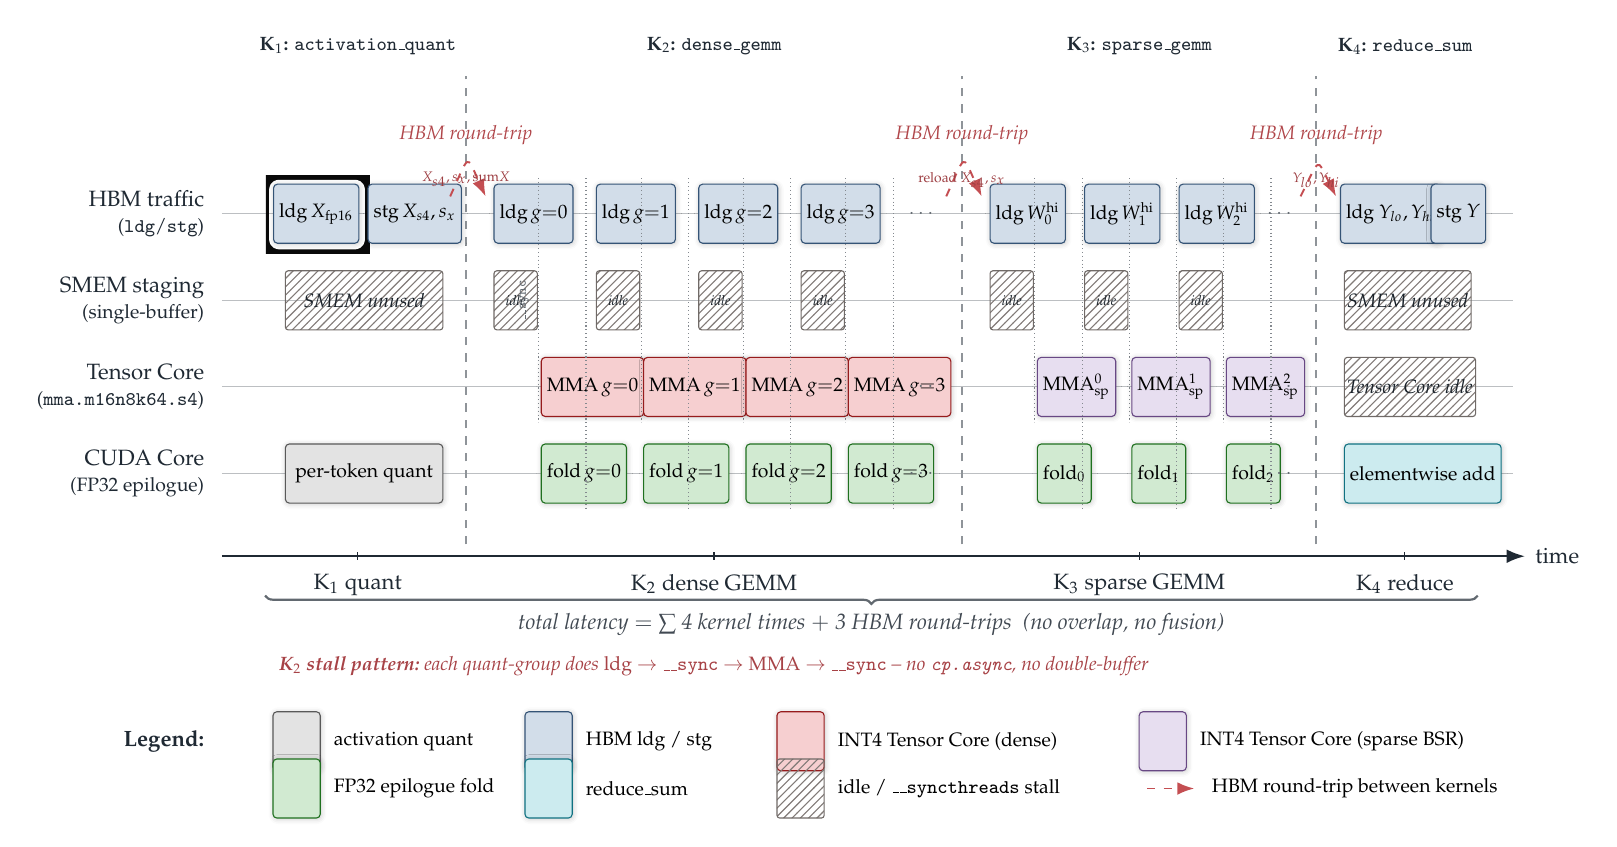
\begin{tikzpicture}[x=1cm, y=1cm]

% =====================================================================
% layout constants
% =====================================================================
% lane y-coordinates (top to bottom)
\def\LHBM{3.6}          % HBM traffic (global memory load / store)
\def\LSM{2.5}           % SMEM staging
\def\LTC{1.4}           % Tensor Core / compute
\def\LEP{0.3}           % epilogue / writeback

% phase column starts (each kernel launch block)
\def\Kqs{0.4}           \def\Kqe{2.75}      % activation_quant_naive
\def\Kds{3.15}          \def\Kde{9.05}      % dense_gemm_naive
\def\Kss{9.45}          \def\Kse{13.55}     % sparse_gemm_naive
\def\Krs{13.95}         \def\Kre{15.80}     % reduce_sum_naive

% =====================================================================
% lane guides + lane labels
% =====================================================================
\foreach \y in {\LHBM, \LSM, \LTC, \LEP} {
  \draw[lane] (-0.15, \y) -- (16.25, \y);
}
\node[lanelab] at (-0.25,\LHBM) {HBM traffic\\{\scriptsize (\texttt{ldg}/\texttt{stg})}};
\node[lanelab] at (-0.25,\LSM)  {SMEM staging\\{\scriptsize (single-buffer)}};
\node[lanelab] at (-0.25,\LTC)  {Tensor Core\\{\scriptsize (\texttt{mma.m16n8k64.s4})}};
\node[lanelab] at (-0.25,\LEP)  {CUDA Core\\{\scriptsize (FP32 epilogue)}};

% =====================================================================
% kernel-boundary shading (light alternating bands behind each kernel)
% =====================================================================
\begin{scope}[on background layer]
  \fill[axisC!4,  rounded corners=2pt] (\Kqs,-0.25) rectangle (\Kqe,4.40);
  \fill[axisC!7,  rounded corners=2pt] (\Kds,-0.25) rectangle (\Kde,4.40);
  \fill[axisC!4,  rounded corners=2pt] (\Kss,-0.25) rectangle (\Kse,4.40);
  \fill[axisC!7,  rounded corners=2pt] (\Krs,-0.25) rectangle (\Kre,4.40);
\end{scope}

% kernel-name captions (top)
\node[font=\scriptsize\bfseries, anchor=south, text=axisC]
  at ({(\Kqs+\Kqe)/2}, 5.50) {\textsc{K}$_1$: \texttt{activation\_quant}};
\node[font=\scriptsize\bfseries, anchor=south, text=axisC]
  at ({(\Kds+\Kde)/2}, 5.50) {\textsc{K}$_2$: \texttt{dense\_gemm}};
\node[font=\scriptsize\bfseries, anchor=south, text=axisC]
  at ({(\Kss+\Kse)/2}, 5.50) {\textsc{K}$_3$: \texttt{sparse\_gemm}};
\node[font=\scriptsize\bfseries, anchor=south, text=axisC]
  at ({(\Krs+\Kre)/2}, 5.50) {\textsc{K}$_4$: \texttt{reduce\_sum}};

% dashed boundaries between kernels
\foreach \x in {\Kqe,\Kde,\Kse} {
  \draw[boundaryLine] (\x+0.20, -0.60) -- (\x+0.20, 5.35);
}

% =====================================================================
%  K1  : activation_quant_naive
%   HBM:   load X_fp16            -> store X_s4 + scale_x + sum_X
%   TC :   (unused)
%   EP :   per-token scalar quant on CUDA cores
% =====================================================================
\node[blkHBM, minimum width=10mm, anchor=west] (qL)
  at (\Kqs+0.10, \LHBM) {ldg\,$X_{\mathrm{fp16}}$};
\node[blkHBM, minimum width=11mm, anchor=west] (qS)
  at (\Kqs+1.30, \LHBM) {stg\,$X_{s4},s_x$};

\node[blkQ, minimum width=20mm, anchor=west] (qC1)
  at (\Kqs+0.25, \LEP) {per-token quant};

% sync stall in SMEM lane (no staging actually happens -- grey strip)
\node[blkStall, minimum width=20mm, anchor=west]
  at (\Kqs+0.25, \LSM) {SMEM unused};

% =====================================================================
%  K2  : dense_gemm_naive   -- four quant-group iterations shown
%   pattern per group g:
%     LDG W,X  ->  __syncthreads  ->  MMA  ->  __syncthreads
%   Single-buffered: next LDG cannot start until MMA finishes.
% =====================================================================
% four iteration columns inside K2
\def\Kdg{1.30}          % width per group iteration (approx)
\foreach \g [count=\i from 0] in {0,1,2,3} {
  \pgfmathsetmacro{\xa}{\Kds + 0.15 + \i*\Kdg}
  \pgfmathsetmacro{\xb}{\xa + 0.55}     % LDG end
  \pgfmathsetmacro{\xc}{\xb + 0.05}     % MMA start (after sync)
  \pgfmathsetmacro{\xd}{\xc + 0.55}     % MMA end

  % HBM lane: LDG W, X, scale, zero, sum_X (read fresh every group!)
  \node[blkHBM, minimum width=5.5mm, anchor=west]
    at (\xa, \LHBM) {\scriptsize ldg\,$g{=}\g$};

  % SMEM lane: single-buffer staging -- drawn as grey "idle" when MMA active
  \node[blkStall, minimum width=5.5mm, anchor=west, font=\tiny\itshape]
    at (\xa, \LSM) {idle};

  % sync barrier tick between LDG and MMA
  \draw[syncTick] (\xb+0.025, \LHBM+0.45) -- (\xb+0.025, \LTC-0.45);
  \ifnum\i=0
    \node[font=\tiny, text=axisC!70, anchor=south, rotate=90]
      at (\xb+0.025, \LSM) {\texttt{\_\_sync}};
  \fi

  % TC lane: MMA over group g
  \node[blkTC, minimum width=5.5mm, anchor=west]
    at (\xc, \LTC) {\scriptsize MMA\,$g{=}\g$};

  % EP lane: scalar FP32 fold -- sequential, after MMA of this group
  \node[blkFP, minimum width=5.5mm, anchor=west]
    at (\xc, \LEP) {\scriptsize fold\,$g{=}\g$};

  % sync barrier after MMA (before next ldg can overwrite smem)
  \draw[syncTick] (\xd+0.025, \LHBM+0.45) -- (\xd+0.025, \LEP-0.45);
}
% ellipsis for remaining groups
\node[font=\scriptsize, text=axisC!70] at (\Kde-0.30, \LHBM) {$\cdots$};
\node[font=\scriptsize, text=axisC!70] at (\Kde-0.30, \LTC)  {$\cdots$};
\node[font=\scriptsize, text=axisC!70] at (\Kde-0.30, \LEP)  {$\cdots$};

% "no cp.async, no double-buffer" annotation -- placed BELOW axis lanes
\node[font=\scriptsize\itshape, text=rtC!85!black, anchor=north]
  at ({(\Kds+\Kde)/2}, -1.90)
  {\textbf{K$_2$ stall pattern:}\ each quant-group does \emph{ldg $\to$ \texttt{\_\_sync} $\to$ MMA $\to$ \texttt{\_\_sync}}\ --\ no \texttt{cp.async}, no double-buffer};

% =====================================================================
%  K3  : sparse_gemm_naive   -- similar stall pattern, on BSR blocks
% =====================================================================
\def\Ksg{1.20}
\foreach \b [count=\i from 0] in {0,1,2} {
  \pgfmathsetmacro{\xa}{\Kss + 0.15 + \i*\Ksg}
  \pgfmathsetmacro{\xb}{\xa + 0.55}
  \pgfmathsetmacro{\xc}{\xb + 0.05}
  \pgfmathsetmacro{\xd}{\xc + 0.55}

  \node[blkHBM, minimum width=5.5mm, anchor=west]
    at (\xa, \LHBM) {\scriptsize ldg\,$W^{\mathrm{hi}}_{\b}$};
  \node[blkStall, minimum width=5.5mm, anchor=west, font=\tiny\itshape]
    at (\xa, \LSM) {idle};
  \draw[syncTick] (\xb+0.025, \LHBM+0.45) -- (\xb+0.025, \LTC-0.45);
  \node[blkSP, minimum width=5.5mm, anchor=west]
    at (\xc, \LTC) {\scriptsize MMA$_{\mathrm{sp}}^{\b}$};
  \node[blkFP, minimum width=5.5mm, anchor=west]
    at (\xc, \LEP) {\scriptsize fold$_{\b}$};
  \draw[syncTick] (\xd+0.025, \LHBM+0.45) -- (\xd+0.025, \LEP-0.45);
}
\node[font=\scriptsize, text=axisC!70] at (\Kse-0.25, \LHBM) {$\cdots$};
\node[font=\scriptsize, text=axisC!70] at (\Kse-0.25, \LTC)  {$\cdots$};
\node[font=\scriptsize, text=axisC!70] at (\Kse-0.25, \LEP)  {$\cdots$};

% =====================================================================
%  K4  : reduce_sum_naive
% =====================================================================
\node[blkHBM, minimum width=10mm, anchor=west]
  at (\Krs+0.10, \LHBM) {\scriptsize ldg $Y_{lo},Y_{hi}$};
\node[blkHBM, minimum width=6mm, anchor=west]
  at (\Krs+1.25, \LHBM) {\scriptsize stg $Y$};
\node[blkRED, minimum width=16mm, anchor=west]
  at (\Krs+0.15, \LEP) {elementwise add};
\node[blkStall, minimum width=16mm, anchor=west, font=\scriptsize\itshape]
  at (\Krs+0.15, \LSM) {SMEM unused};
\node[blkStall, minimum width=16mm, anchor=west, font=\scriptsize\itshape]
  at (\Krs+0.15, \LTC) {Tensor Core idle};

% =====================================================================
%  HBM round-trip arrows between kernels
%  (the defining cost of the unfused baseline)
% =====================================================================
% K1 -> K2 : X_s4, scale_x, sum_X flushed to HBM, reloaded by K2
\draw[rtArrow] (\Kqe, \LHBM+0.22)
  .. controls +(0.25, 0.55) and +(-0.25, 0.55) .. (\Kds+0.05, \LHBM+0.22);
\node[font=\scriptsize\itshape, text=rtC!90!black, anchor=south, align=center]
  at ({(\Kqe+\Kds)/2}, \LHBM+0.75)
  {HBM round-trip};
\node[font=\tiny, text=rtC!80!black, anchor=north, align=center]
  at ({(\Kqe+\Kds)/2}, \LHBM+0.65)
  {$X_{s4},s_x,\mathrm{sum}X$};

% K2 -> K3 : Y_low materialised in HBM (not consumed here but dense finalises)
\draw[rtArrow] (\Kde, \LHBM+0.22)
  .. controls +(0.25, 0.55) and +(-0.25, 0.55) .. (\Kss+0.05, \LHBM+0.22);
\node[font=\scriptsize\itshape, text=rtC!90!black, anchor=south, align=center]
  at ({(\Kde+\Kss)/2}, \LHBM+0.75)
  {HBM round-trip};
\node[font=\tiny, text=rtC!80!black, anchor=north, align=center]
  at ({(\Kde+\Kss)/2}, \LHBM+0.65)
  {reload $X_{s4},s_x$};

% K3 -> K4 : Y_low + Y_high reloaded for add
\draw[rtArrow] (\Kse, \LHBM+0.22)
  .. controls +(0.25, 0.50) and +(-0.25, 0.50) .. (\Krs+0.05, \LHBM+0.22);
\node[font=\scriptsize\itshape, text=rtC!90!black, anchor=south, align=center]
  at ({(\Kse+\Krs)/2}, \LHBM+0.75) {HBM round-trip};
\node[font=\tiny, text=rtC!80!black, anchor=north, align=center]
  at ({(\Kse+\Krs)/2}, \LHBM+0.65) {$Y_{lo},Y_{hi}$};

% =====================================================================
%  time axis
% =====================================================================
\draw[->, thick, axisC] (-0.15,-0.75) -- (16.40,-0.75)
  node[right, font=\footnotesize] {time};

\foreach \xa/\xb/\lbl in {%
  \Kqs/\Kqe/{K$_1$ quant},%
  \Kds/\Kde/{K$_2$ dense GEMM},%
  \Kss/\Kse/{K$_3$ sparse GEMM},%
  \Krs/\Kre/{K$_4$ reduce}%
} {
  \pgfmathsetmacro{\xc}{(\xa + \xb)/2}
  \draw[axisC] (\xc,-0.70) -- (\xc,-0.80);
  \node[font=\footnotesize, anchor=north, text=axisC] at (\xc,-0.85) {\lbl};
}

% wasted-time bracket above axis (emphasises serialised launches)
\draw[decorate, decoration={brace, amplitude=3pt, mirror}, axisC!70, thick]
  (\Kqs,-1.25) -- (\Kre,-1.25);
\node[font=\footnotesize\itshape, text=axisC!85, anchor=north]
  at ({(\Kqs+\Kre)/2},-1.35)
  {total latency $=$ $\sum$ 4 kernel times $+$ 3 HBM round-trips\ \  (no overlap, no fusion)};

% =====================================================================
%  legend (bottom, two rows)
% =====================================================================
\def\LyA{-3.10}
\def\LyB{-3.70}
\node[font=\footnotesize\bfseries, anchor=east, text=axisC] at (-0.25,\LyA) {Legend:};

% row A
\node[blkQ,   minimum width=6mm] at (0.80,\LyA) {};
\node[anchor=west, font=\scriptsize] at (1.15,\LyA) {activation quant};
\node[blkHBM, minimum width=6mm] at (4.00,\LyA) {};
\node[anchor=west, font=\scriptsize] at (4.35,\LyA) {HBM ldg / stg};
\node[blkTC,  minimum width=6mm] at (7.20,\LyA) {};
\node[anchor=west, font=\scriptsize] at (7.55,\LyA) {INT4 Tensor Core (dense)};
\node[blkSP,  minimum width=6mm] at (11.80,\LyA) {};
\node[anchor=west, font=\scriptsize] at (12.15,\LyA) {INT4 Tensor Core (sparse BSR)};

% row B
\node[blkFP,  minimum width=6mm] at (0.80,\LyB) {};
\node[anchor=west, font=\scriptsize] at (1.15,\LyB) {FP32 epilogue fold};
\node[blkRED, minimum width=6mm] at (4.00,\LyB) {};
\node[anchor=west, font=\scriptsize] at (4.35,\LyB) {reduce\_sum};
\node[blkStall, minimum width=6mm] at (7.20,\LyB) {};
\node[anchor=west, font=\scriptsize] at (7.55,\LyB) {idle / \texttt{\_\_syncthreads} stall};
\draw[rtArrow] (11.60,\LyB) -- (12.20,\LyB);
\node[anchor=west, font=\scriptsize] at (12.30,\LyB) {HBM round-trip between kernels};

\end{tikzpicture}
\end{document}
